\chapter{General Kernel Spectral Method}
\label{chap:general-kernel-spectral-method}

Now that we know how to treat power law potentials in the construction of a spectral method for the solution of equilibrium measures, can we consider more general kernels as well?
The approach in this chapter is to expand a general kernel $K$ in a power law basis and utilise the methodology introduced in the previous chapter to construct a general kernel spectral method.

\section{Expansion of the General Kernel}
More specifically, one choice of basis that could be made is the basis of monomials (so integer powers of the power law kernel basis).
Using standard methods from function approximation theory, we expand the general kernel $K: \R^+ \to \R$ in the basis of $G$ Jacobi polynomials (cf. \Cref{def:jacobi-polynomials})
$$K(r) \approx \sum_{l=0}^{G-1} \tilde{g_l} P_l^{(a, b)}\left(2 r^2 - 1\right)\,, \quad \vec{\tilde{g}} := (\tilde{g}_0, ..., \tilde{g}_{G-1})^T \in \R^G\,,$$
which we then reproject into the monomial basis to obtain the monomial coefficients $g_l \in \R$ such that
\begin{equation}
  K_G(r) = \sum_{l=0}^{G-1} g_l r^l \approx K(r)\,,\quad \vec{g} := ({g}_0, ..., {g}_{G-1})^T \in \R^G\,.
  \label{eq:monomial-expansion}
\end{equation}

% \subsection{Reprojection from Radial Jacobi Polynomials}
For versatility in the choice of basis, we obtain the monomial coefficients of a given kernel $K(r)$ by $\vec{g} = B \vec{\tilde{g}}$, where $B \in \R^{G \times G}$ is the conversion matrix between the basis of radial Jacobi polynomials and the basis of monomials.
The basis conversion matrix $B$ is easily obtained by projection of each monomial into the Jacobi basis, more specifically the $k$th column ($k \in \N_0$) is comprised of the Jacobi coefficients of $r^{k}$.

% Does reprojection from Jacobi to monomials make sense / is it better for stability etc.?
% If so, explain reprojection using basis transformation matrix. --> yes.

\section{Description of the Method}
Given the ansatz in \Cref{eq:ansatz}, the total energy of the equilibrium measure (cf. \Cref{def:equilibrium-measure}) is given by
\begin{align*}
  U_{K_G}[\hat{\rho}] & = \iint K_G\left(\norm{\hatvec{x}-\hatvec{y}}\right) \,\dd\hat{\rho}(\hatvec{x})\dd\hat{\rho}(\hatvec{y})
  = \sum_{l=0}^{G-1} g_l \iint \norm{\hatvec{x}-\hatvec{y}}^l \,\dd\hat{\rho}(\hatvec{x})\dd\hat{\rho}(\hatvec{y})                \\
                      & = R^{2d} \sum_{l=0}^{G-1} g_l R^l \iint \norm{\vec{x}-\vec{y}}^l \,\dd\rho(\vec{x})\dd\rho(\vec{y})
  = R^{2d} \sum_{l=0}^{G-1} g_l R^l U^{(l)}[\rho]\,,
\end{align*}
using \Cref{def:power-law-potential}.
The \textit{general kernel operator} $\mathcal{Q}_G: \functionspace \to \functionspace$, analogous to $\mathcal{Q}_{\alpha,\beta}$ for the attractive-repulsive case, is given by
\begin{align*}
  \mathcal{Q}_G[\hat{\rho}](\hatvec{x}) & := \int_{B_R(\vec{0})} K_{G}\left(\norm{\hatvec{x} - \hatvec{y}}\right) \hat{\rho}(\hatvec{y}) \,\dd\hatvec{y}
  = \int_{B_R(\vec{0})} \sum_{l=0}^{G-1} g_l \norm{\hatvec{x}-\hatvec{y}}^l \hat{\rho}(\hatvec{y}) \,\dd\hatvec{y}                                       \\
                                        & = \sum_{l=0}^{G-1} g_l R^{l+d} \int_{B_1(\vec{0})} R^l\norm{\vec{x} - \vec{y}}^l \rho(\vec{y}) \,\dd\vec{y}
  = \sum_{l=0}^{G-1} g_l R^{l+d} \mathcal{Q}^l[\rho](\vec{x})\,,
\end{align*}
where $\mathcal{Q}^l \in \R^{N \times N}$ is the power law operator (cf. \Cref{def:power-law-operator}).
Its matrix representation $Q_G$ acting on coefficient space is derived analogously from $Q^\beta \in \R^{N \times N}$.

The solution process then follows analogously from \Cref{chap:spectral-method}.
A spy plot of the full operator may be found in \Cref{fig:morse-operator}, resulting solutions in \Cref{fig:morse-solution-increasing-order}.

\paragraph{Choice of the Jacobi Basis:}
As for the attractive-repulsive case, the radial Jacobi basis $\jacobi[k]{x}$ requires two parameters $a, b > -1$ (cf. \Cref{def:jacobi-polynomials} and \Cref{thm:jacobi-orthogonality-condition}).
In the attractive-repulsive case, these are chosen based on $\alpha$, some $m \in N_0$ and the dimension $d$.
Our method chooses the most dominant monomial power in the expansion ($l_{\rm dom} = \max_{l \in \{0, ..., G-1\}} |g_l|$) in place of $\alpha$ to obtain $a = m - \frac{l_{\rm dom} + d}{2}$.
This choice once again places a restriction on either $l_{\rm dom} < G$ and therefore $G$, or on the parameter $m \in \N_0$.
That is, $-d < l_{\rm dom} < 2 + 2m - d$.
This is to ensure that the most dominant contribution to the operator is exactly banded (as established in \Cref{sec:derivation-of-operator}), making the full operator $Q_G$ as diagonally dominant as possible.
The second parameter remains $b = \frac{d-2}{2}$.

\begin{figure}[H]
  \centering
  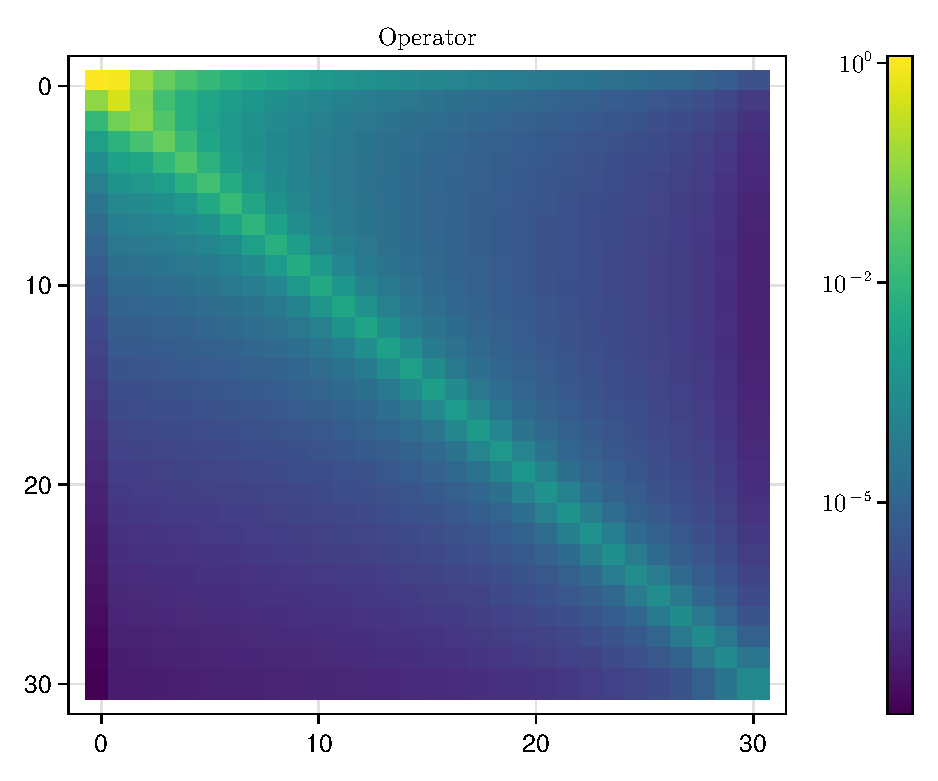
\includegraphics[width=0.5\linewidth]{results/morse/full-operator.pdf}
  \caption[Full Morse operator]{The full operator constructed from the $G=8$th order monomial expansion $K_G$ of the Morse potential function $K_{C_a, l_a, C_r, l_r}(r)$ with parameters as given above.}
  \label{fig:morse-operator}
\end{figure}

Solutions for the Morse potential can be found in \Cref{fig:morse-solution-increasing-order} for varying order $N$, solutions for varying order $G$ (the number of terms in the polynomial expansion of the kernel $K(r)$) are depicted in \Cref{fig:monomial-solutions}.

\begin{figure}[H]
  \centering
  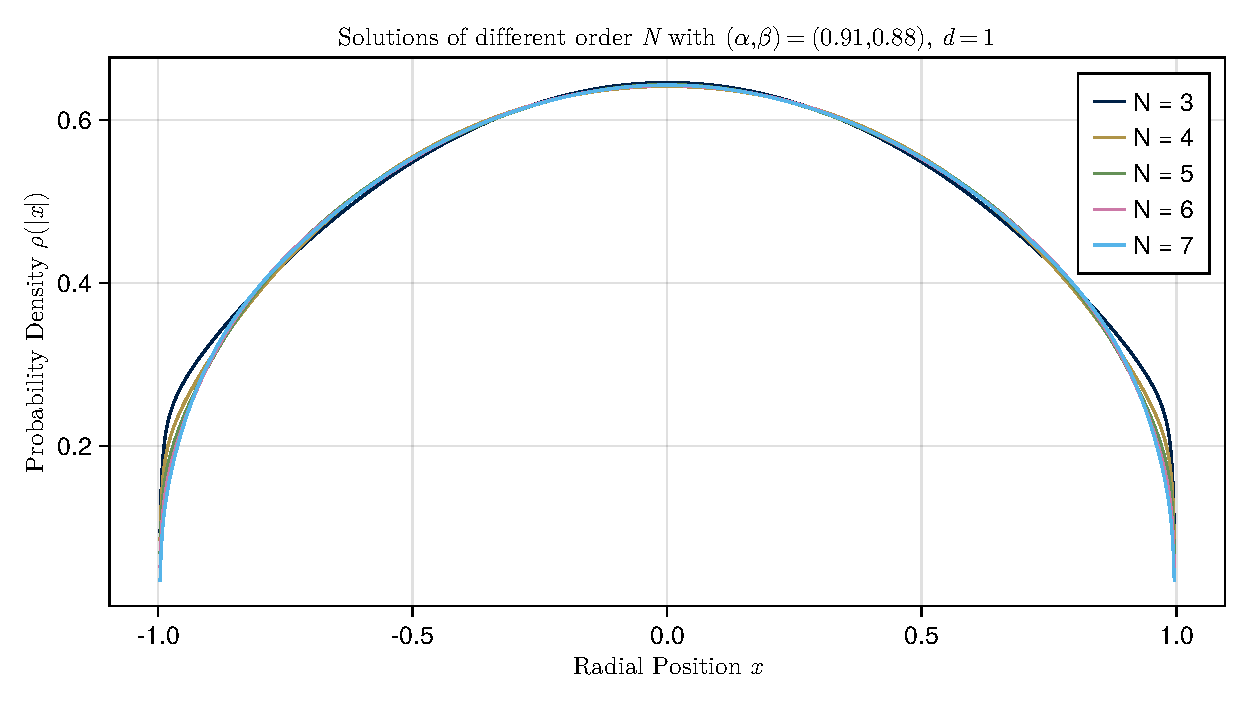
\includegraphics[width=0.8\linewidth]{results/morse/solution-increasing-order.pdf}
  \caption[General kernel solutions of increasing order]{Solutions $\rho_N(x)$ of increasing order $N$ in the general kernel setting with a monomial expansion of highest order $G = 8$ of the Morse potential $K_{C_a, l_a, C_r, l_r}(r)$.}
  \label{fig:morse-solution-increasing-order}
\end{figure}

Instead of increasing the order of the expansion in the solution ansatz (cf. \Cref{eq:ansatz}), one can increase the expansion order of the general kernel, $G$ to ensure a good match between the general kernel expansion and $K_G(r)$.

\begin{figure}[H]
  \centering
  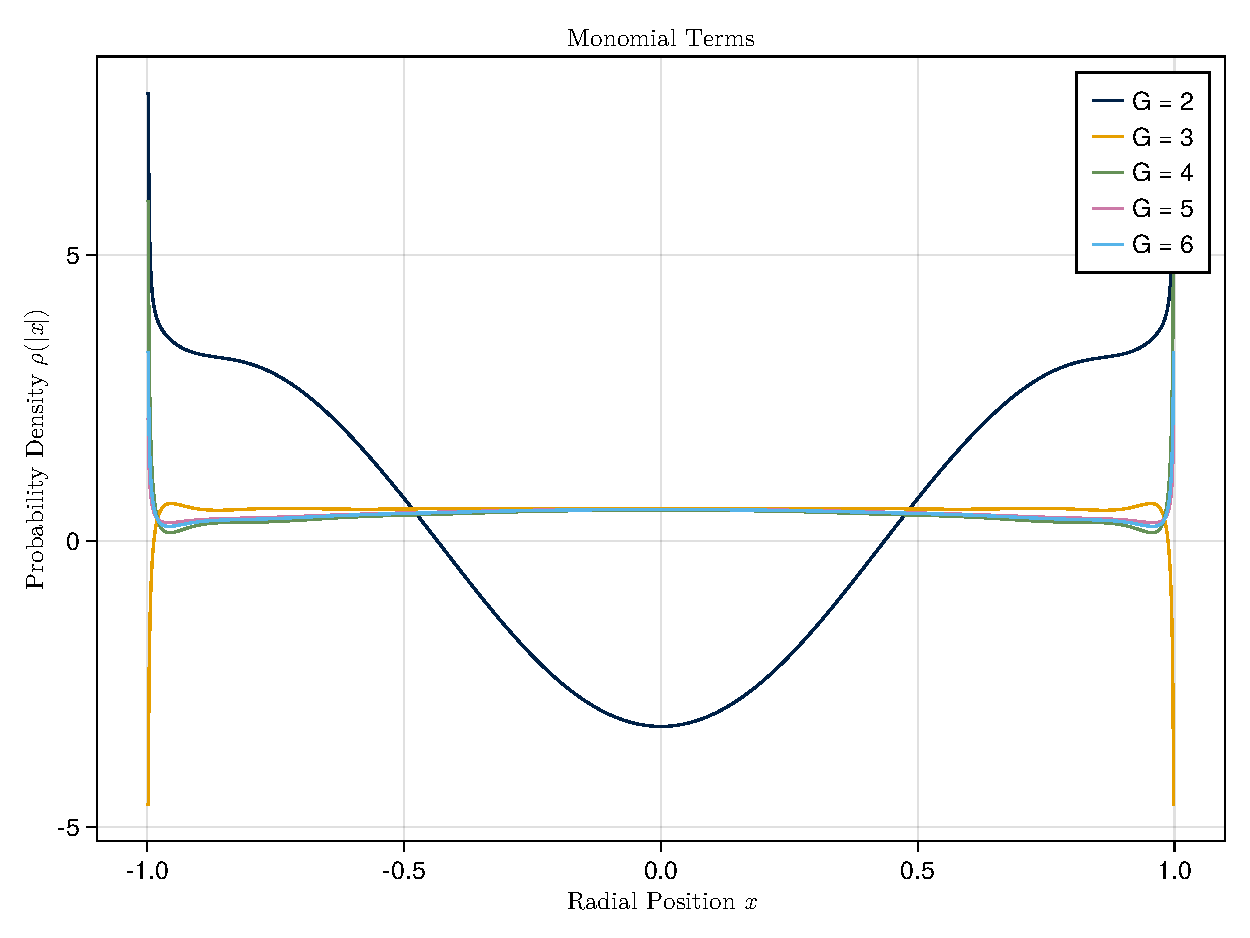
\includegraphics[width=0.8\linewidth]{results/morse/monomial-solutions.pdf}
  \caption[General kernel solutions with varying $G$]{Solutions $\rho_8(x)$ for an increasing number of terms $G$ in the monomial expansion of a general kernel $K$, in this case given by the Morse potential $K_{C_a, l_a, C_r, l_r}(r)$. So each solution $\rho_8(x)$ is a linear combination of $8$ Jacobi polynomials together with a weight, cf. \Cref{eq:ansatz}. The singularities of lower order solutions disappear for higher $G$, which extensive simulation results attest.}
  \label{fig:monomial-solutions}
\end{figure}

As one can see, the solutions improve the better the approximation of the general kernel $K$ becomes with growing order $G$ of its monomial expansion.
\Cref{fig:monomial-basis-convergence} illustrates this behaviour by showing the rapid improvement of the squared error for growing order $G$.

\begin{figure}[H]
  \centering
  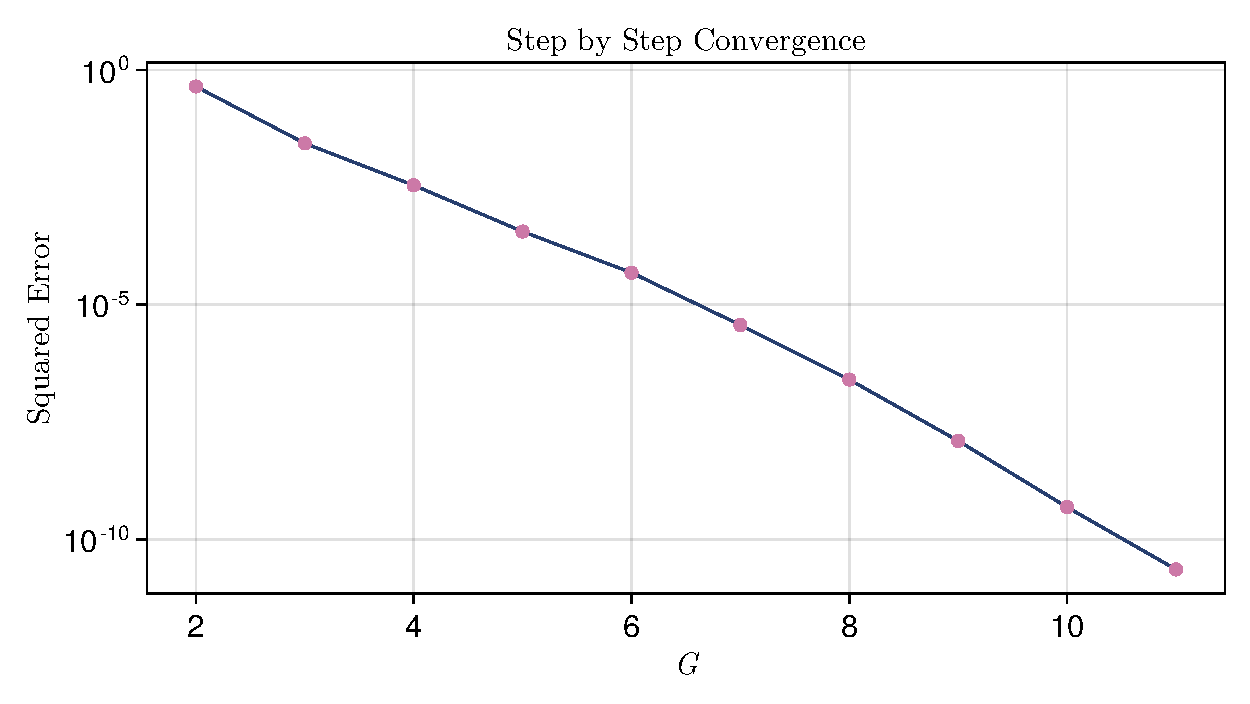
\includegraphics[width=0.7\linewidth]{results/morse/monomial-basis-convergence.pdf}
  \caption[Step-by-step convergence when increasing the degree of the monomials]{
    Convergence of numerical solutions $\rho_N(x)$ as compared to $\rho_{24}(x)$, visualised using the squared error of the pointwise evaluation of both functions in $200$ points.
    The solver again uses $K(r) = K_{C_a, l_a, C_r, l_r}(r)$.
  }
  \label{fig:monomial-basis-convergence}
\end{figure}

Solutions for varying support radius $R$ can be found in \Cref{fig:varying-R-solutions}.

\begin{figure}[H]
  \centering
  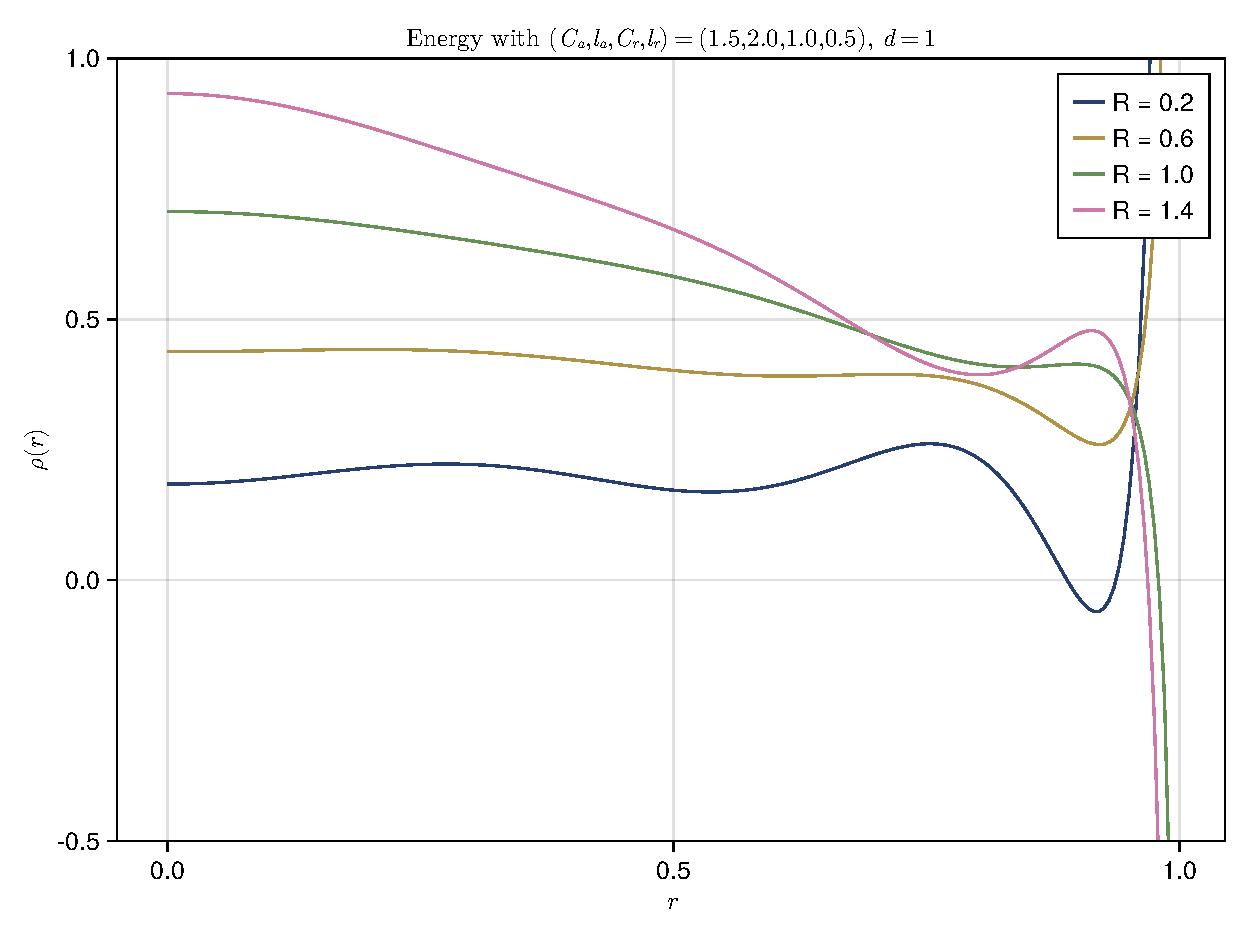
\includegraphics[width=0.7\linewidth]{results/morse/varying-R-solutions.pdf}
  \caption[Solutions with varying $R$]{General kernel solutions ($N = 6$, $G = 8$) with varying $R$ when using the Morse potential $K_{C_a, l_a, C_r, l_r}(r)$ with parameters as given above.}
  \label{fig:varying-R-solutions}
\end{figure}
